% relay whitepaper: one page. Build: see README.md in this folder.
\documentclass[9pt,a4paper]{extarticle}
\usepackage[a4paper,top=10mm,bottom=10mm,left=14mm,right=14mm]{geometry}
\usepackage[T1]{fontenc}
\usepackage[sc]{mathpazo}
\usepackage[scaled=0.9]{helvet}
\usepackage{amsmath,amssymb}
\usepackage{microtype}
\usepackage{graphicx}
\usepackage{multicol}
\usepackage{xcolor}
\usepackage{enumitem}
\usepackage[hidelinks]{hyperref}
\usepackage{titlesec}

\definecolor{ink}{HTML}{0B0B0B}
\definecolor{ink2}{HTML}{52514E}
\definecolor{accent}{HTML}{2A78D6}
\color{ink}
\hypersetup{pdftitle={Relay: running coding-agent plans across usage windows},pdfauthor={cube-digital}}

\setlength{\columnsep}{6mm}
\setlength{\parindent}{0pt}
\setlength{\parskip}{1.8pt}
\linespread{1.0}
\titleformat{\section}{\sffamily\bfseries\fontsize{9.4}{11}\selectfont}{\color{accent}\thesection}{0.5em}{}
\titlespacing*{\section}{0pt}{4pt}{1.2pt}
\setlist{nosep,leftmargin=1.05em,labelsep=0.45em}
\newcommand{\para}[1]{\textsf{\textbf{#1}}\enspace}
\pagestyle{empty}

\begin{document}

{\sffamily\bfseries\fontsize{15.5}{18}\selectfont Relay: running coding-agent plans across usage windows\par}
\vspace{2pt}
{\sffamily\small\color{ink2} cube-digital \enspace·\enspace relay v0.1.2 \enspace·\enspace October 2026 \enspace·\enspace \href{https://github.com/cube-digital/relay}{github.com/cube-digital/relay}\par}
\vspace{5pt}

{\small Relay is a plugin for Claude Code and Codex. It turns a written plan into parallel work for the cheapest model that can do each task, and keeps the plan running across the five-hour usage windows of a Pro or Max subscription for as long as it takes. Before a run it predicts the agents, worktrees, windows and hours the plan needs; after a run it learns the account's real rates from usage readings stamped into the run's ledger.\par}

\vspace{4pt}
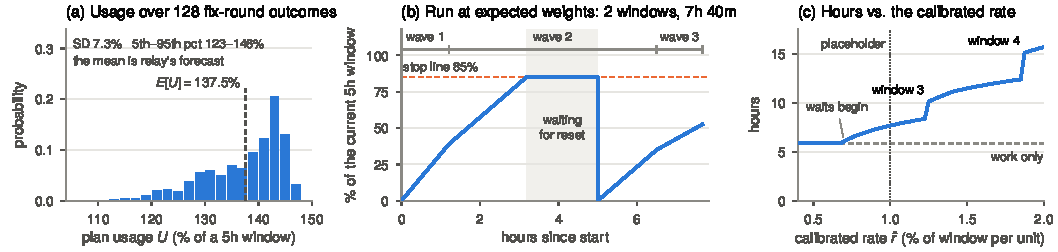
\includegraphics[width=\textwidth]{figure.pdf}
{\footnotesize\color{ink2} \textbf{Figure 1.} The 30-task example plan (\textsf{docs/whitepaper/example-plan.md}: 7 lanes, 3 waves, 108.4 units of work, 137.5 expected with fix rounds) at the placeholder rates $r=1\%$ and $m=4$\,min per unit. (a)~Usage over all $2^7$ fix-round outcomes, exact, drawn in 2-point bins; its mean, 137.5\%, is the forecast. (b)~The run at expected lane weights reaches the stop line during wave~2, pauses 1\,h\,49\,min for the reset and finishes in window~2: 5\,h\,51\,min of work, 7\,h\,40\,min in total. (c)~The rate decides how long a run waits, not how long it works; waits begin near $\hat r=0.68$ and each jump is one more window. Computed by \textsf{data.mjs} with relay's model code.\par}
\vspace{1pt}

\begin{multicols}{2}
\fontsize{8.7}{10.4}\selectfont

\section{The problem we started from}
A Pro or Max subscription meters Claude Code in a five-hour window and a weekly limit; a long plan runs into the window and waits for someone to come back. Multi-agent runs use about 15× the tokens of a chat~[1], and a subagent started without a model inherits the session's, Opus by default on Pro and Max~[2], although most of a plan does not need Opus. Agents also test too much and too weakly: re-running unchanged tests appears in 50--83\% of agent tasks~[3], 80\% of agent-written test patches have weak or no oracles~[4], and prescribing TDD inside the loop cost 3--8.5× the tokens with no measured gain in a small sample~[5]. The goal: the most finished, reviewed work per window, and plans that run for twenty hours unattended.

\section{Mechanism}
\begin{itemize}
\item \para{Plans carry the decisions.} Every task has a tier (cheap, mid, strong: Haiku, Sonnet, Opus, or the Codex equivalents), a risk, files, dependencies, a test budget and a narrow \emph{done} check; judgment is spent once, when planning.
\item \para{Lanes and waves, computed, not prompted.} Tasks touching the same files are joined (union-find), cycles between groups collapse, chains fold up to six tasks; waves are longest-path levels. A wave holds at most four lanes, each in its own git worktree, one commit per task.
\item \para{Budget gates.} At 60\% of the window (80\% of the week) new agents of every role but the architect start on mid instead of strong. At 85\% (95\%) none is exempt and no new implementer or test agent starts; lanes in flight finish with the agents they have, clean work merges, a handoff is written. A mod enforces this in Claude Code; in Codex the skills ask for it.
\item \para{Small contexts.} Workers return at most 6--15 lines by role, the rest goes to report files; the ledger on disk survives compaction; a \emph{marathon} is a chain of fresh headless sessions that resume from the ledger and wait out each reset.
\item \para{QA, not test volume.} Tests come from the spec within a per-task budget; a hook refuses the same test command on unchanged code; no agent can edit protected acceptance tests.
\end{itemize}

\section{The model}
\para{Weights.} Task $t$ weighs $w_t=T(\text{tier}_t)\,R(\text{risk}_t)$ with $T=(1,3,7)$ and $R=(0.8,1,1.4)$; lane $l$ weighs $W_l=\sum_{t\in l}w_t$.

\para{Fix rounds.} Lane $l$ needs a fix round ($B_l=1$) with probability $p_l\in\{0.2,0.5,0.8\}$, set by its riskiest task and independent of other lanes; the round re-works $\kappa=0.35$ of the lane. With $r$ the share of the window per unit, the plan uses
\begin{gather*}
U=r\sum_l W_l(1+\kappa B_l),\qquad \mathrm{E}[U]=r\sum_l \widetilde W_l,\\
\widetilde W_l=W_l(1+\kappa p_l),\qquad \mathrm{Var}[U]=r^2\kappa^2\sum_l W_l^2\,p_l(1-p_l).
\end{gather*}
The forecast is $\mathrm{E}[U]$ with its standard deviation; Fig.~1a is the exact distribution. The count of lanes needing a fix, $F=\sum_l B_l$, is Poisson-binomial with $\mathrm{E}[F]=\sum_l p_l=4.7$. Later rounds, reviews and orchestration inside a wave are not modeled per lane; once calibrated, $r$ contains them. The final review, after the last wave, is outside the model.

\para{Waves.} Wave $k$ has expected weight $\widetilde W_k=\sum_{l\in k}\widetilde W_l$, is expected to use $\bar U_k=r\widetilde W_k$ of the window and lasts $\tau_k=m\,C_k$ minutes, where $C_k$ is the makespan of its $\widetilde W_l$ on $P=4$ slots. With at most four lanes per wave, $C_k=\max_{l\in k}\widetilde W_l$.

\para{Windows.} A walk at the expected weights: a wave starts whenever the window is below the stop line $u^*=85\%$; usage and time accrue linearly within a wave; at $u^*$ the run pauses until the reset and the rest of the wave continues in the next window; a window also ends five hours after it opens. A live budget reading sets the starting usage and the current reset; Fig.~1b starts from an empty window. Averaged over all 128 outcomes the walk also gives 7\,h\,40\,min here.

\para{Calibration.} A ledger line carries the latest reading, if under 20 minutes old, and the window's reset time, e.g.\ \textsf{[5h 23.4\% resets 16:30 · 7d 41\%]}. Wave $k$, from the previous wave's last merge line to its own, yields $r_k=\Delta U_k/\widetilde W_k$ and $m_k=\Delta t_k/C_k$ (a weekly rate likewise). A wave without readings at both ends, or containing a reset (the start stamp's reset time passed, or the reading fell), is skipped. Over the waves kept, the estimates are ratio estimators,
\[
\hat r=\frac{\sum_k \Delta U_k}{\sum_k \widetilde W_k}=\frac{\sum_k \widetilde W_k r_k}{\sum_k \widetilde W_k},\qquad \hat m=\frac{\sum_k \Delta t_k}{\sum_k C_k}.
\]
The same $\widetilde W$ is used to learn $\hat r$ and to forecast, so fix rounds count once. Each rate replaces its placeholder ($r=1\%$, $m=4$\,min) from its first sample; from three waves, the plan's usage at $\min_k r_k$ and $\max_k r_k$ is shown too. The usage, windows and time lines say when they rest on a placeholder.

\section{What is not claimed}
\begin{itemize}
\item The five-hour window is crossed, not avoided. The weekly limit is the real ceiling; the forecast says when a plan does not fit what is left of it.
\item $T$, $R$, $p_l$ and $\kappa$ are priors, not fitted. $r$ and $m$ are shared by all tiers and fixed for the run, although the 60\% gate moves work to cheaper models. Lanes are independent and do not contend. Real lanes front-load usage, so the stop line comes earlier than the linear walk says, while agents in flight run past it; the walk ignores the weekly stop line. Skipped waves are not a random sample, so $\hat r$ and $\hat m$ may be biased. Readings come from the Claude Code mod only: Codex runs stay on placeholders.
\item Savings are not measured yet. Next: per-tier rates by non-negative least squares, $\Delta U_k\approx\sum_j c_j W_{k,j}$ over tiers $j$, once about ten waves exist; bootstrap intervals; an A/B benchmark of the same plans with plain Claude Code, superpowers and relay, scored as \% of a window per merged task at equal mutation score.
\end{itemize}

\vspace{1pt}
{\scriptsize\color{ink2}
[1]~Anthropic, \emph{How we built our multi-agent research system}, 2025.
[2]~Claude Code docs: sub-agents, model configuration.
[3]~arXiv:2609.30725. [4]~arXiv:2606.18168.
[5]~B.~Böckeler, \emph{TDD in the agent loop}, martinfowler.com.
Sources for every design decision: \textsf{docs/design.md}. Rebuild this page: \textsf{docs/whitepaper/README.md}.\par}

\end{multicols}
\end{document}
